\chapter{章节标题}
\section{二级标题}
\subsection{三级标题}
\subsubsection{四级标题}

% 描述列表,可以指定描述词
描述列表:
\begin{description}
    \item[1.] (非负性)$d(x,y)\geqslant 0$且$d(x,y)=0\Leftrightarrow x=y$
    \item[2.] (对称性)$d(x,y)=d(y,x)$
    \item[3.] (三角不等式)$d(x,y)\leqslant d(x,z)+d(y,z)$
\end{description}

% 有序列表
有序列表:
\begin{enumerate}
    \item (非负性)$d(x,y)\geqslant 0$且$d(x,y)=0\Leftrightarrow x=y$
    \item (对称性)$d(x,y)=d(y,x)$
    \item (三角不等式)$d(x,y)\leqslant d(x,z)+d(y,z)$
\end{enumerate}

% 无序列表
无序列表:
\begin{itemize}
    \item $\textbf{n维欧氏空间} R^n$\\
          定义距离$d=(\sum_{k=1}^{n}\left | \xi _k-\eta _k\right
              |^2)^{1/2}$或者$d=\underset{1\leqslant k\leqslant n}{max}\left | \xi _k-\eta
              _k\right |$
    \item $\textbf{空间C[a,b]}$\\
          定义距离$d=\underset{a\leqslant t\leqslant  b }{max}\left | x(t)-y(t)\right |$
    \item $\textbf{空间L}^\infty$\\
          先回顾一下空间$L^\infty$:\begin{equation*}
              \left \| f\right \|_\infty=inf\begin{Bmatrix}
                  M:\left | f\right |\leqslant M \quad a.e. \quad on\quad  E
              \end{Bmatrix}
          \end{equation*}
          \begin{equation*}
              L^\infty(E)=\begin{Bmatrix}
                  f:f${在E可测}$ \left \| f\right \|_\infty< \infty		\end{Bmatrix}
          \end{equation*}
          定义距离$d=\underset{mF_0=0,F_0\subset F}{inf}\begin{Bmatrix}
                  \underset{t\in F \setminus F_0}{sup}\left | x(t)-y(t)\right |
              \end{Bmatrix}$
\end{itemize}

% 定义环境示例
\begin{definition}
    内容.
\end{definition}

% 注记环境示例
\begin{note}
    注意了.
\end{note}

% 定理环境示例
\begin{theorem}[($\textbf{唯一性}$)]
    $x_n \to x,x_n \to y\Rightarrow x=y$.
\end{theorem}

% 证明环境示例
\begin{myproof}
    $0\leqslant d(x,y)\leqslant d(x_n,x)+d(x_n,y)\to 0$,根据夹逼定理,$d(x,y)=0 \Rightarrow x=y$
\end{myproof}

% 例题环境示例
\begin{problem}
微分方程解的存在性与唯一性:微分方程\begin{equation*}
    \left\{\begin{matrix}
        \frac{dy}{dx}=p(x,y) \\
        y(x_0)=y_0
    \end{matrix}\right.
\end{equation*}
其中$f\in C(\mathbb{R}^2)$\\
设$y$满足Lipschitz条件,即$\exists K>0,s.t.$\begin{equation*}
    \left | f(x,y)-f(x,y')\right | \leqslant K\left | y-y'\right |
\end{equation*}
\end{problem}

% 题解环境示例
\begin{solution}
    \begin{align*}
        y(x)-y_0 & =\int_{x_0}^{x}\frac{dy}{dx}dx \\
                 & =\int_{x_0}^{x}f(x,y(x))dx     \\
                 & =\int_{x_0}^{x}f(t,y(t))dt
    \end{align*}
    (可以看出这个解的结构但无法说明解的存在性与唯一性,但是积分不一定收敛)

    取$\delta >0,s.t. k\delta <1$,在$C[x_0-\delta,x_0+\delta]$上定义T:\begin{equation*}
        (Ty)(x)=y_0+\int_{x_0}^{x}f(t,y(t))dt
    \end{equation*}
\end{solution}

% 性质环境示例
\begin{property}[(有界性)]
    内容.
\end{property}

% 引理环境示例
\begin{lemma}
    内容.
\end{lemma}

% 推论环境示例
\begin{corollary}
    内容.
\end{corollary}

% 图片引入及引用
如图 \ref{1} 所示.

\begin{figure}[htbp]
    \centering % 居中
    
\includegraphics[scale=0.2]{Ali.jpg} % 引入图片
    \caption{this is Ali} % 图片标题
    \label{1} % 标签
\end{figure}

% 表格定义及引用
如表 \ref{table:1} 所示.

\begin{table}[htbp]
    \caption{表格标题}
    \label{table:1} % 标签

    % 定义表格格式
    \centering % 居中

    % 表格内容
    \begin{tabular}{| l | c | c | r |} % | 表示垂直线,p 表示宽度,l 表示左对齐,c 表示居中对齐,r 表示右对齐
        \hline % 水平线
        \multicolumn{4}{|c|}{Country List}                                       \\ % 多列合并
        \hline
        Country Name or Area Name & ISO ALPHA 2 Code & ISO ALPHA 3 & ISO ALPHA 4 \\
        \hline
        Afghanistan               & AF               & AFG         & abcd        \\
        \hline
    \end{tabular}
\end{table}

% 函数图像示例
\begin{tikzpicture}[thick]
    \def\U{*0.027*\textwidth}
    % 绘制坐标轴
    \draw[-{Stealth}](-2\U,0)--(18\U,0) coordinate[label={right:$x$}];
    \draw[-{Stealth}](0,-2\U)--(0,13\U) coordinate[label={above:$y$}];
    % 设定坐标点
    \path
    coordinate(x) at (11\U,0)
    coordinate(y) at (0,7\U)
    coordinate(c) at (11\U,7\U)
    coordinate(c1) at (7\U,5\U)
    coordinate(c2) at (15\U,9\U);
    \draw[dashed](y)--(c)--(x);
    % 绘制曲线
    \draw(7\U,5\U) cos(11\U,7\U) sin(15\U,9\U);
    % 绘制各点标签
    \draw
    (y)node[dot,label={left:$y$}]{}
    (c)node[dot]{}
    (x)node[dot,label={below:$x$}]{}
    (0,0)node[dot,label={below left:$0$}]{};
\end{tikzpicture}

% 几何图像示例
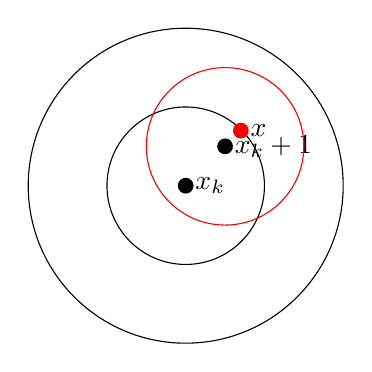
\begin{tikzpicture}
    \draw (0,0) circle(2);
    \fill (0,0) circle (.1);
    \node at (0,0) [right] {$x_k$};
    \draw (0,0) circle(1);
    \fill (0.5,0.5) circle (.1);
    \node at (0.5,0.5) [right] {$x_k+1$};
    \draw[red] (0.5,0.5) circle(1);
    \fill[red](0.7,0.7) circle (.1);
    \node at (0.7,0.7) [right] {$x$};
\end{tikzpicture}

% 引用参考文献
引文.\upcite{1}

\begin{property}[(可列可加性)]
    内容.
\end{property}

\begin{theorem}
    内容.
\end{theorem}

\chapter{第二章}

\begin{theorem}
    内容.
\end{theorem}

\setcounter{propertyname}{0}
\begin{property}
    内容.
\end{property}

\begin{property}[(非负性)]
    内容.
\end{property}

% 参考文献
\bibliography{books}